\documentclass[a4paper, 12pt]{article}%тип документа



%отступы
\usepackage[left=1cm,right=1cm,top=1cm,bottom=2cm,bindingoffset=0cm]{geometry}

%%% Работа с русским языком
\usepackage{graphicx}
\usepackage{cmap}                           % поиск в PDF
\usepackage{mathtext} 			 	       % русские буквы в формулах
\usepackage[T2A]{fontenc}               % кодировка
\usepackage[utf8]{inputenc}              % кодировка исходного текста
\usepackage[english,russian]{babel} 
\usepackage{float}
\usepackage{sidecap}
\usepackage{graphicx}
\usepackage{wrapfig}
\usepackage{multirow}
\usepackage[export]{adjustbox} % локализация и переносы
\usepackage[unicode, pdftex]{hyperref}
\usepackage{subfig}% http://ctan.org/pkg/subfig
\usepackage{booktabs}

\usepackage{wrapfig}


%Матеша
\usepackage{amsmath,amsfonts,amssymb,amsthm,mathtools} % AMS
\usepackage{icomma} % "Умная" запятая

%\mathtoolsset{showonlyrefs=true} % Показывать номера только у тех формул, на которые есть \eqref{} в тексте.

%% Шрифты
\usepackage{euscript}	 % Шрифт Евклид
\usepackage{mathrsfs} % Красивый матшрифт

%% Свои команды
\DeclareMathOperator{\sgn}{\mathop{sgn}}

%% Перенос знаков в формулах (по Львовскому)
\newcommand*{\hm}[1]{#1\nobreak\discretionary{}
	{\hbox{$\mathsurround=0pt #1$}}{}}
\newcommand{\rref}[1]{(\ref{#1})}
\newenvironment{comment}{}{}
\newcommand{\picref}[1]{рис. \ref{#1}}
\newcommand{\mbf}{\mathbf}
\newcommand{\Equip}[3]{
	
	{\bf #1:} $\Delta = \pm #2$ \si{#3}}
\newcommand{\equip}[1]{
	
	{\bf #1}}

%\usepackage{caption}
%\usepackage{subcaption}


\author{Гаврилин Илья Дмитриевич \\
		Добровольская  Ксения Дмитриевна\\_{}
	Б01-101}
\title{\textbf{Лабораторная работа 4.3.3\\ 
		Исследование разрешающей способности микроскопа методом Аббе}}
	
\begin{document}
	\maketitle
	\section{Аннотация}
	
	В данной работе проводится определение периода решёток по их пространственному спектру и по увеличенному изображению, а также определение дифракционного предела разрешения объектива микроскопа методом Аббе. Кроме того, исследуются пространственная фильтрация и мультипликация изображения решётки.
	
	\section{Теоретические сведения}
	
	\paragraph{Принцип двойной дифракции и формирование оптического	изображения.}
	
	Формирование изображения с помощью линзы можно рассматривать, основываясь на идее пространственного спектрального разложения. Монохроматическую волну, идущую от предмета, представим в виде суперпозиции плоских волн разных направлений $ \alpha $, т. е. разных пространственных частот $ u = k \sin \alpha $. Каждая гармоника фокусируется линзой в определённую точку фокальной плоскости, и там возникает картина пространственного спектра. По этой причине фокальную плоскость линзы называют фурье-плоскостью.
	
	В процессе распространения света от предмета до фурье-плоскости осуществляется преобразование Фурье светового поля (по терминологии Аббе -- первая дифракция). Процесс распространения света от фурье-плоскости до плоскости изображения (рис. \ref{fig:screenshot1}) -- вторая дифракция.
	
	Можно сказать, что в процессе образования изображения происходит два последовательных преобразования Фурье: от входной плоскости $ П_1 $ к фурье-плоскости -- первая дифракция, и затем от фурье-плоскости с помощью линзы $ Л_2 $ к выходной плоскости $ П_2 $ -- вторая дифракция.
	
	\begin{figure}[H]
		\centering
		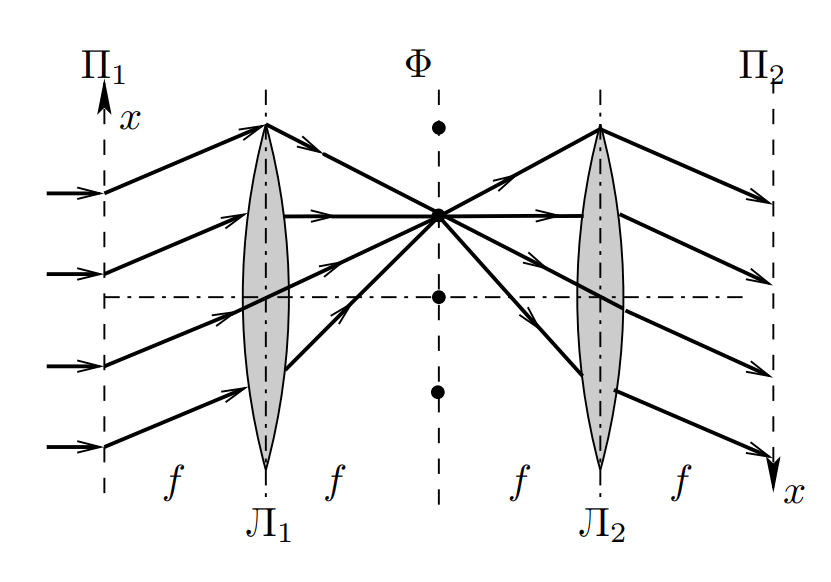
\includegraphics[width=0.7\linewidth]{Screenshot_1}
		\caption{Двойная дифракция Аббе}
		\label{fig:screenshot1}
	\end{figure}
	
	\paragraph{Пространственная фильтрация.}
	
	В фурье-плоскости возможно избирательное воздействие на разные пространственные гармоники: установив в любой точке $ x $ этой плоскости пластинку, вносящую определённое поглощение, мы изменим амплитуду и фазу плоской волны с пространственной частотой $ u = k x / f $, не изменяя амплитуд и фаз других плоских волн.
	
	\paragraph{Мультипликация изображения.}
	
	Изображение, возникающее в плоскости $ П_2 $, представляет собой периодически повторяющееся с периодом $$ d_0 = \lambda f / d $$ изображение объекта с функцией пропускания $ f_0 (x) $.
	Соседние элементы периодической структуры, видимой в $ П_2, $ $ f(x) = \Sigma f_0(x-n d_0) $, не налагаются друг на друга при условии $ d_0 > a $, где $ a $ -- размер объекта. Число элементов $ N $ размноженного изображения определяется шириной главного максимума картины дифракции Фраунгофера на отдельной щели решётки: $$ N\approx 2 b / d_0. $$
	
	\paragraph{Разрешающая способность. Критерий Рэлея.} 
	
	Согласно качественному критерию, предложенному Рэлеем, два источника света различимы, если дифракционный максимум одного приходится на минимум другого. Т. е, расстояние между центрами пятен $ \Delta x $ равно полуширине пятна Эйри (рис. \ref{fig:screenshot2}): \[\Delta x = 1.22 \frac{\lambda}{D} z,\] где $ z $ -- расстояние от диафрагмы до плоскости наблюдения, а $ D $ -- диаметр диафрагмы. Отсюда минимальное угловое разрешение равно: \[\alpha_{min} \approx 1.22 \frac{\lambda}{D}.\]
	
	\begin{figure}[H]
		\centering
		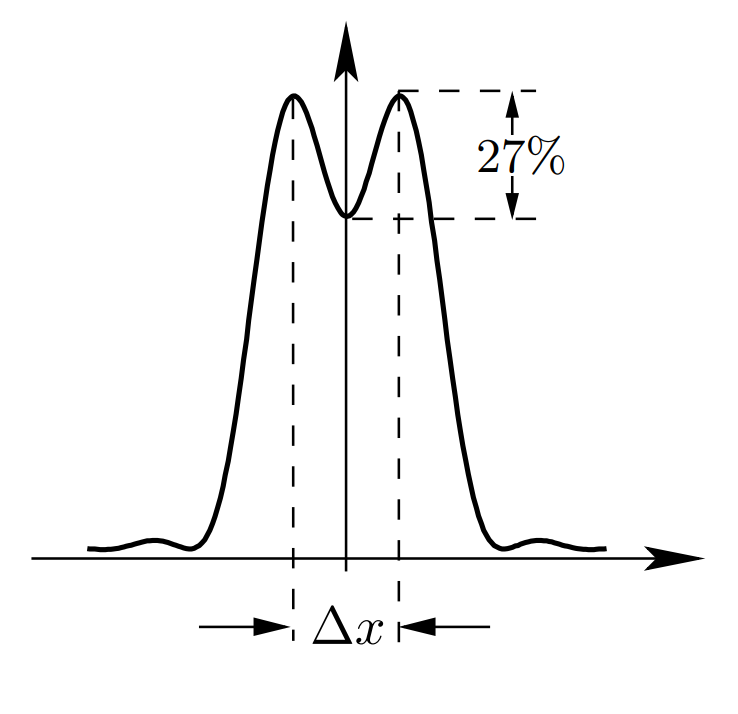
\includegraphics[width=0.5\linewidth]{Screenshot_2}
		\caption{Разрешение двух пятен Эйри}
		\label{fig:screenshot2}
	\end{figure}
	
	
	\subsection{Расчётные формулы}
	
	\begin{figure}[H]
		\centering
		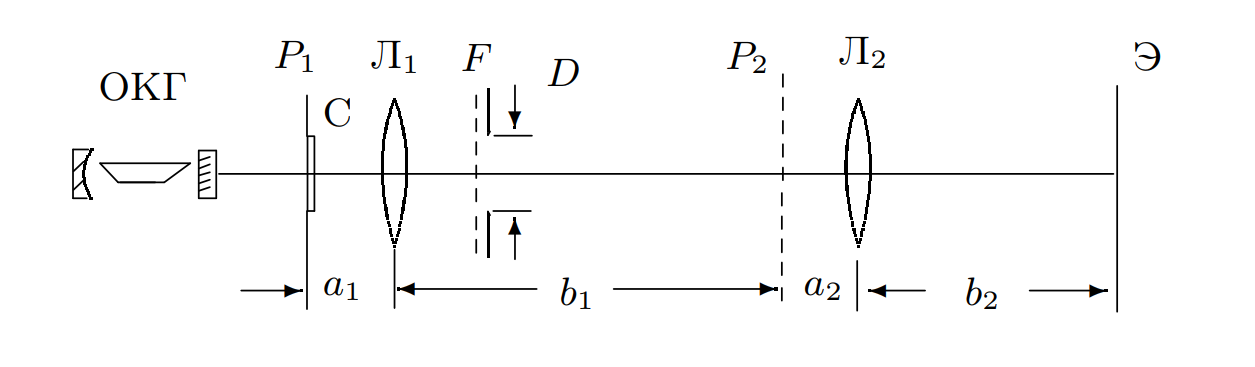
\includegraphics[width=0.8\linewidth]{Screenshot_3}
		\caption{Схема экспериментальной установки}
		\label{fig:screenshot3}
	\end{figure}
	Минимально разрешаемое объективом расстояние:
	\begin{equation}\label{минимальное_расстояние}
		l_{min}\approx \frac{2 f \lambda}{D},
	\end{equation}
	где $ f $ -- фокусное расстояние линзы.
	
	Условия главных максимумов:
	\begin{equation}\label{условие_максимумов}
		d \sin \theta_x = m_x \lambda, \;\;\;	d \sin \theta_y = m_y \lambda,
	\end{equation}
	где $ m_{x, y} $ -- порядок дифракционных максимумов.
	
	Увеличение системы собирающих линз (в условиях опыта):
	\begin{equation}\label{увеличение}
		\Gamma = \frac{b_1 b_2}{a_1 a_2},
	\end{equation}
	где $ a, \; b $ -- соответствующие расстояния на рис. \ref{fig:screenshot3}.
	\section{Ход работы}
	\subsection{Определение периода решеток по пространственному спектру}
	В этой части рассчитывается период решеток по дифракционной картине получаемой на экране. На экране наблюдаем дифракционную картину состоящую из точек. Возьмем ось $x$ и на ней отсчитаем $N$ максимумов. В таблице рассчитаем период решеток.\\
	Замер производим на расстоянии между решеткой и экраном $L = 144\pm1$ см, длина волны излучения лазера $\lambda = 532$ нм.
	\begin{table}[H]
		\centering
		\begin{tabular}{|l|c|c|c|c|c|c|}
			\hline
			№ решетки       & 1    & 2     & 3     & 4    & 5     & 6     \\ \hline
			$l$, мм       & 235  & 248   & 263   & 234  & 249   & 264   \\ \hline
			$N-1$, макс.     & 3    & 8     & 17    & 3    & 8     & 17    \\ \hline
			$d, \cdot 10^{-6}$ м       & 9.78 & 24.71 & 49.52 & 9.82 & 24.61 & 49.33 \\ \hline
			$\delta d, \cdot 10^{-6}$ м & 0.4  & 1.5   & 2.8   & 0.4  & 1.5   & 2.8   \\ \hline
		\end{tabular}
		\caption{Период решетки по пространственному спектру}
		\label{ref:table1}
	\end{table} 
	По определенному порядку решетки (таблица \ref{ref:table1}) поймем что верхний и нижний ряд решеток идентичен, поэтому в дальнейшем будем исследовать три решетки из верхнего ряда, обозначенные цифрами.
	\subsection{Определение периода решетки по изображению, полученному при помощи микроскопа}
	Соберем микроскоп по схеме рис. \ref{fig:screenshot3}, замерим характерные расстояния и сразу из длины тубуса получим все параметры микроскопа.\\
	\begin{center}
		$f_2 = 25$ мм;$f_1 = 110$ мм\\
	
	$a_1 = 14\pm1$ см;$a_2 = 2.5\pm0.1$ см\\
	$b_1 = 77.5\pm1$ см;$b_2 = 51\pm1$ см\\
	Вычислим увеличение: Г$ = 113\pm7$\\
	\end{center}
	Отсюда найдем период решетки по увеличенному изображению решетки, при этом не трогая компоновку системы и сохраняя увеличение нашего микроскопа.
	\begin{table}[H]
		\centering
		\begin{tabular}{|l|c|c|c|}
			\hline
			№ решетки & 1    & 2     & 3     \\ \hline
			l, мм & 27   & 28    & 28    \\ \hline
			N-1, макс. & 29   & 12    & 6     \\ \hline
			$d, \cdot 10^{-6}$ м. & 8.25 & 20.67 & 41.33 \\ \hline
		\end{tabular}
	\caption{Определение периода решетки по увеличенному изображению}
	\end{table}
	\subsection{Определение периода решетки по разрешающей способности}
	Сохраним схему из прошлого эксперимента, только в фокальную плоскость первой линзы на рис. \ref{fig:screenshot3} установим регулируемую щель. Регулируя щель будем добиваться пропадания на изображении части полос, по микрометрическому винту определим ширину щели.
	\begin{table}[H]
		\centering
		\begin{tabular}{|l|c|c|c|}
			\hline
			№ решетки & 1 & 2     & 3     \\ \hline
			D, мм & - & 4.1   & 2.3   \\ \hline
			$d, \cdot 10^{-6}$ м. & - & 28.29 & 50.43 \\ \hline
		\end{tabular}
		\caption{Период решетки по разрешающей способности}
	\end{table}
	Несмотря на то что полученных точек мало, попробуем построить зависимость периода решетки от обратной ширины щели.
	\begin{figure}[H]
		\centering
		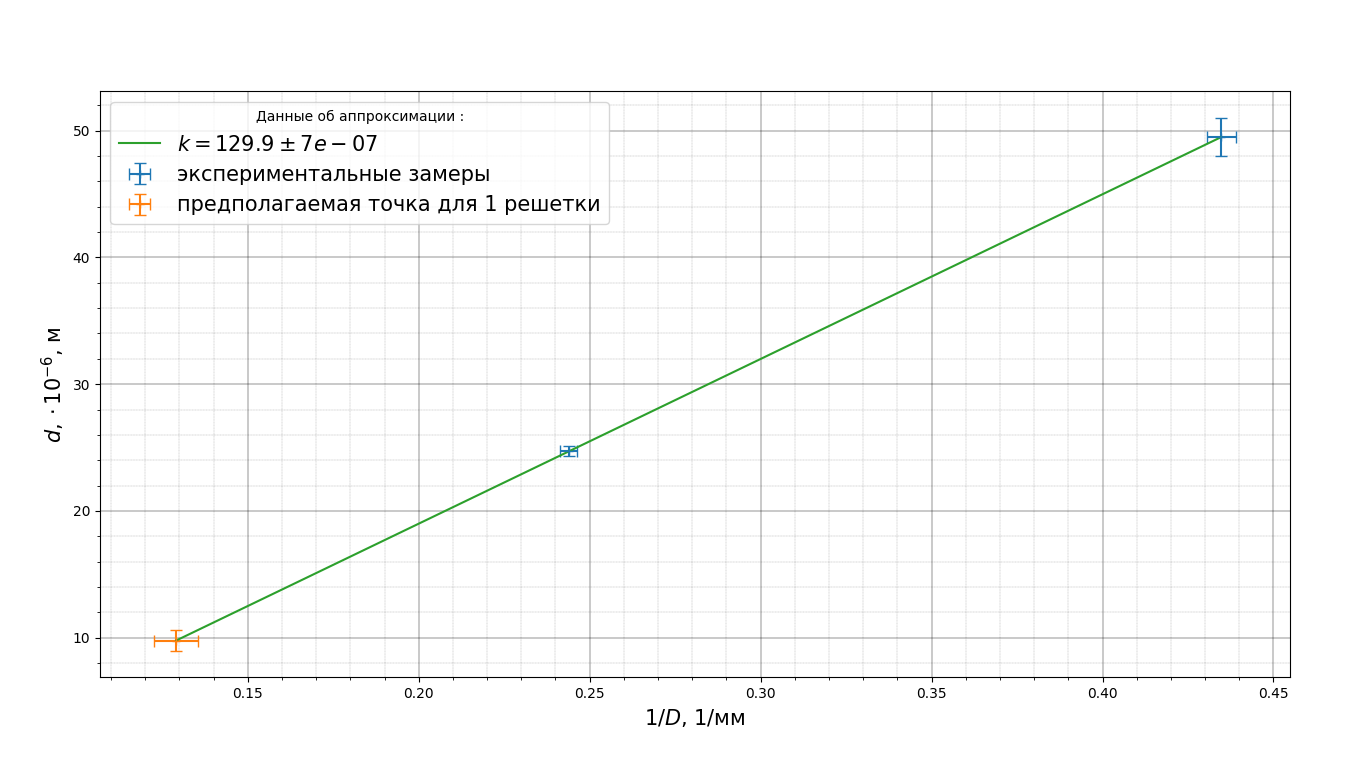
\includegraphics[width=0.8\linewidth]{зависимость}
		\caption{Зависимость периода решетки от обратной ширины щели ($d = f(1/D)$)}
		\label{fig:}
	\end{figure}
	\subsection{Пространственная фильтрация изображения}
	Провели опыт по пространственной фильтрации изображения. Установив ширину щели так чтобы оставить только один ряд максимумов, получали соответственно изображения только горизонтальных или только вертикальных ребер решетки (в зависимости от поворота щели). Также установив щель под углом 45\% к вертикали получили полосы наклоненные на тот же самый угол. Замерили расстояния между полосами для каждого из положений: \\
	\begin{table}[H]
		\centering
		\begin{tabular}{|l|c|c|c|}
			\hline
			$\alpha$ & 45  & 90 & 0  \\ \hline
			L, мм & 50  & 50 & 50 \\ \hline
			N     & 15  & 10 & 10 \\ \hline
			l, мм & 3.3 & 5  & 5  \\ \hline
		\end{tabular}
		\caption{Расстояние между полосами}
	\end{table}
	Получили расстояния одинаковые для 0 и 90 градусов, а для 45 градусов показания в $\sqrt{2}$ раз меньше.
	\subsection{Проверка теории Аббе}
	По рис. 4 получили зависимость $d = f(1/D)$, аппроксимируя ее прямой линией можем получить коэффициент наклона:\\
	\begin{center}
		$k_{exp} = 129.9$\\
	\end{center}
	Рассчитав данный коэффициент теоретически получили:\\
	\begin{center}
			$k_{th} = 120$\\
	\end{center}
	Получили сходные оценки коэффициентов, что говорит справедливости теории Аббе.
	\section{Выводы}
	В ходе работы:\\
	1) Получили период решетки тремя разными способами, построили микроскоп\\
	\begin{table}[H]
		\centering
		\begin{tabular}{|c|c|c|c|}
			\hline
			№ & спектр & микроскоп & разреш. способ. \\ \hline
			1 & 9.8    & 8.25      & -               \\ \hline
			2 & 24.71  & 20.67     & 28.29           \\ \hline
			3 & 49.52  & 41.33     & 50.43           \\ \hline
		\end{tabular}
	\caption{Период решеток в зависимости от метода замера ([$\cdot 10^{-6} $ м] )}
	\end{table}
	2) Построили зависимость периода решетки от обратной ширины щели, получили характерный коэффициент наклона этой зависимости.\\
	3) По  полученному ранее коэффициенту проверили справедливость теории Аббе.
\end{document}